\documentclass[letterpaper,12pt,fleqn]{article}
\usepackage{matharticle}
\pagestyle{empty}
\newcommand{\norm}[1]{\left\|#1\right\|}
\newcommand{\inner}[2]{\left<#1,#2\right>}
\newcommand{\conj}[1]{\overline{#1}}
\renewcommand{\O}{\Omega}
\newcommand{\p}{\rho}
\newcommand{\mc}{\mathcal{C}}
\begin{document}
\section*{Hilbert Spaces}

\begin{definition}
  A \emph{Hilbert} space is a complete inner product space.
\end{definition}

\begin{examples}
  \listbreak
  \begin{enumerate}
  \item Finite dimensional: $\C^N$ where $\inner{z}{w}=\sum_{k=1}^Nz\conj{w}$.

  \item Infinite dimensional: $\ell^2$ where
    $\inner{x}{y}=\sum_{k=1}^{\infty}x_k\conj{y_k}$.

  \item Infinite dimensional: $L^2(\O)$ where
    $\inner{f}{g}=\int_{\O}f\conj{g}$.
  \end{enumerate}
\end{examples}

Non-Hilbert inner product spaces arise from:
\begin{enumerate}
\item The norm is not induced by an inner product.
\item The space is not complete.
\end{enumerate}

\begin{examples}
  \listbreak
  \begin{enumerate}
  \item $\mc[a,b]$ where $\inner{f}{g}=\int_a^bf\conj{g}$.

    Consider the counterexample $f_n=t^n\in\mc[0,1]$:

    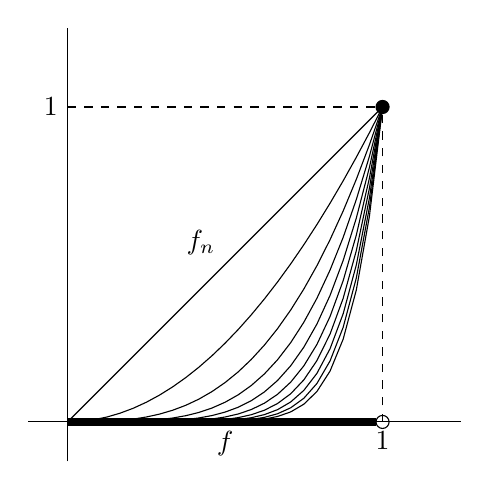
\begin{tikzpicture}
      \draw (-0.5,0) -- (5,0);
      \draw (0,-0.5) -- (0,5);
      \node [below] at (4,0) {$1$};
      \node [left] at (0,4) {$1$};
      \draw [dashed] (0,4) -- (4,4);
      \draw [dashed] (4,0) -- (4,4);
      \draw [domain=0:4] plot ({\x},{\x});
      \draw [domain=0:4] plot ({\x},{4*(\x/4)^2});
      \draw [domain=0:4] plot ({\x},{4*(\x/4)^3});
      \draw [domain=0:4] plot ({\x},{4*(\x/4)^4});
      \draw [domain=0:4] plot ({\x},{4*(\x/4)^5});
      \draw [domain=0:4] plot ({\x},{4*(\x/4)^6});
      \draw [domain=0:4] plot ({\x},{4*(\x/4)^7});
      \draw [domain=0:4] plot ({\x},{4*(\x/4)^8});
      \draw [domain=0:4] plot ({\x},{4*(\x/4)^9});
      \draw [domain=0:4] plot ({\x},{4*(\x/4)^10});
      \node [draw, circle, scale=0.5] (a) at (4,0) {};
      \node [draw, fill, circle, scale=0.5] (b) at (4,4) {};
      \draw [line width=1mm] (0,0) to (a);
      \node [above left] at (2,2) {$f_n$};
      \node [below] at (2,0) {$f$};
    \end{tikzpicture}

    Claim: $f_n$ is Cauchy:

    AWLOG: $n<m$
    \begin{eqnarray*}
      \norm{f_n-f_m}^2 &=& \int_0^1\abs{f_n-f_m}^2 \\
      &=& \int_0^1(t^n-t^m)^2dt \\
      &=& \int_0^1(t^{2n}-2t^{n+m}+t^{2m})dt \\
      &=& \left[\frac{1}{2n+1}t^{2n+1}-\frac{2}{n+m+1}t^{n+m+1}+
        \frac{1}{2m+1}t^{2m+1}\right]_0^1 \\
      &=& \frac{1}{2n+1}-\frac{2}{n+m+1}+\frac{1}{2m+1} \\
      &\to& 0-0+0 \\
      &=& 0
    \end{eqnarray*}

    Thus, $f_n$ is Cauchy in the norm.

    Claim: $f_n\to f$ where
    $f=\begin{cases}0, & 0\le x<1 \\ 1, & x=1\end{cases}$
    \begin{eqnarray*}
      \norm{f_n-f}^2 &=& \norm{f_n-0}^2 \\
      &=& \norm{f_n}^2 \\
      &=& \int_0^1t^{2n}dt \\
      &=& \left.\frac{1}{2n+1}t^{2n+1}\right|_0^1 \\
      &=& \frac{1}{2n+1} \\
      &\to& 0
    \end{eqnarray*}

    Thus, $f_n\to f$ in the norm; however, $f$ is discontinuous and thus
    $f\notin\mc[0,1]$.

    Therefore, $\mc[0,1]$ is not complete, and thus not Hilbert.

    \bigskip

  \item Let $\ell_0$ be the set of complex sequences $x$ such that only a
    finite number of the $x_k\ne0$, with
    $\inner{x}{y}=\sum_{k=1}^{\infty}x_k\conj{y_k}$.

    Let $x_n=
    \left(1,\frac{1}{2},\frac{1}{3},\ldots,\frac{1}{n},0,0,\ldots\right)$.

    Claim: $x_n$ is Cauchy in the norm:

    AWLOG: $n<m$
    
    \begin{eqnarray*}
      \norm{x_n-x_m}^2 &=& \sum_{k=1}^{\infty}\abs{x_{n_k}-x_{m_k}}^2 \\
      &=& \sum_{k=1}^{\infty}x_{n_k}^2-2x_{n_k}x_{m_k}+x_{m_k}^2 \\
      &=& \sum_{k=1}^{\infty}\left(x_{n_k}^2-2\sum_{k=1}^{\infty}x_{n_k}x_{m_k}+
      \sum_{k=1}^{\infty}x_{m_k}^2\right) \\
      &=& \sum_{k=1}^n\frac{1}{k^2}-2\sum_{k=1}^n\frac{1}{k^2}+
      \sum_{k=1}^m\frac{1}{k^2} \\
      &\to& \frac{\pi^2}{6}-2\frac{\pi^2}{6}+\frac{\pi^2}{6} \\
      &=& 0
    \end{eqnarray*}

    Thus $x_n$ is Cauchy in the norm.

    By letting $m\to\infty$ above, it is clear that
    $x_n\to x=\left(1,\frac{1}{2},\frac{1}{3},\ldots\right)$, the harmonic
    sequence.

    However, $x\notin\l_0$ and so $\ell_0$ is not complete, and therefore
    $\ell_0$ is not Hilbert.
  \end{enumerate}
\end{examples}

\end{document}
